\section{Gibbs oscillation}
Simulate Gibbs oscillation on a given signal $s(t)$.

\subsection*{Background}
The Fourier series of a complex-valued periodic function $s(t)$, integrable over the interval $[a, b]$on the real line, is defined as: 
$$s(t) = \sum _{n=-\infty }^{\infty }c_{n}e^{i2\pi {\tfrac {n}{T}}t}$$

Where $T = b - a$ is the period of function. Fourier coefficients $c_{n}$ are: 
$$c_{n}={\frac {1}{T}}\int _{a}^{b}s(t)\ e^{-i2\pi {\tfrac {n}{T}}t}dt$$


\subsection*{Program}
\importMLCode{code/Q4.m}

\begin{figure*}[ht!]
	\centering
	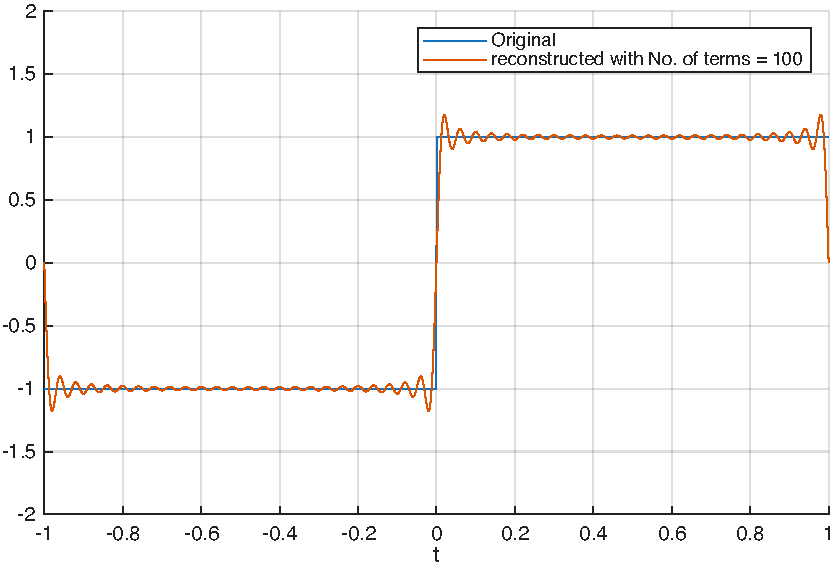
\includegraphics[width=.5\textwidth]{img/Q4.pdf}
	\caption*{Notice the wide oscillation near discontinuities}
\end{figure*}